\documentclass[20pt,a4paper]{report}
\usepackage[T2A,T1]{fontenc}
\usepackage[utf8]{inputenc}
\usepackage{blindtext}
\usepackage[russian]{babel}
\usepackage{mwe}
\usepackage{graphbox}
\usepackage[document]{ragged2e}
\usepackage[margin=50pt]{geometry}
\usepackage{longtable}
\usepackage{fontspec}
\usepackage{float}
\usepackage{titlesec}
\usepackage{setspace}
\usepackage{minted}

\usepackage{hyperref}
\hypersetup{
    colorlinks,
    citecolor=black,
    filecolor=black,
    linkcolor=black,
    urlcolor=black
}

\setstretch{1.5}
\graphicspath{{./images/}}
\setmainfont{LiberationSerif}
\setmonofont{Hack}
\titleformat{\chapter}{\normalfont\LARGE\bfseries}{\thechapter}{1em}{}
\titleclass{\chapter}{straight}
\titlespacing{\chapter}{0pt}{0pt}{5pt}[25pt]


\begin{document}
	\large
	\textbf{РК2; РИП; Сысойкин Егор ИУ5-54Б} \\
	\chapter{Задание}
		Вариант Г.
		\begin{enumerate}
			\item Данные класса 1 должны выводиться в виде таблицы с утолщенными внутренними границами (cellspacing).
			\item Данные класса 2 должны выводиться в виде нумерованного списка.
			\item С использованием технологии CSS реализуйте чересстрочное форматирование(“зебру”) для данных списка.
		\end{enumerate}
		\begin{tabular}{|c|c|c|}
				\hline
				\textbf{№ варианта} & \textbf{Класс 1} & \textbf{Класс 2} \\ \hline
				20 & Деталь & Поставщик \\ \hline
		\end{tabular}

	\chapter{Код}
		\small
		\inputminted[tabsize=4, linenos]{html}{index.html}

	\chapter{Экранные формы}
		\begin{figure}[H]
			\centering
			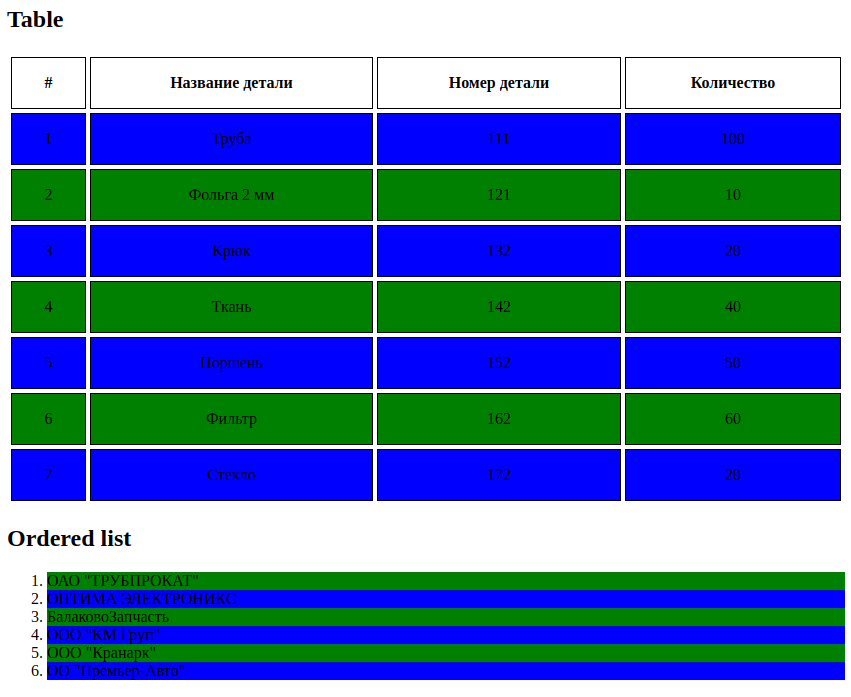
\includegraphics[scale=0.7]{screen.png}
		\end{figure}
\end{document}

